The trend of both curiosity and profit-driven human development has caused a
surge in the amount of openly accessible raw data. More often than not, the data is generated much faster than it can be processed into something interpretable or useful. In the endeavor of keeping up with the inflow of information, there are two major factors that significantly hinder our progress. First, Moore’s law implicitly sets a physical limit to the number of transistors that can be placed on a chip, consequently limiting how powerful and how fast electronic systems can become (barring a paradigm shift in the fundamental design of semiconductors). The second is the Nyquist-Shannon sampling theorem (NST), which limits the range of frequencies a recording device can successfully capture. This states that given that you know a signal's highest frequency component $f_B$, sampling it at a rate $f_S$ that is at least twice this frequency is sufficient to capture all of the pertinent information regarding that signal; that is $f_S \geq 2f_B$, where $f_B$ is known as the Nyquist rate \cite{Shannon1949}, and also as the signal bandwidth. For signals that are not naturally bandlimited, such as images, the ability reproduce a signal is dependent on the device's resolution and still follows the same principle: there should be at least twice the number of pixels codimensional with the image's highest spatial frequency. For practical day-to-day use, the NST covers everything you need. However, issues arise when bandwidth and storage are at a premium. Typically, after sensing a signal, not all of the raw data is stored. Rather, this data is converted to a compressed format by systematically discarding values such that the loss of information is virtually imperceptible. Thus, the process of acquiring massive amounts of data followed by compression is extremely wasteful. Enter compressive sensing.

\section{Compressive sensing}
\label{sec:cs}

Consider a signal $\vec{x} \in \mathbb{R}^{n}$; this notaton indicates that $\vec{x}$ is real-valued (but can easily be extended to complex-valued signals), one-dimensional vector of size $n$. The process of acquisition or sensing this signal can be modeled as a linear system, where the physical signal properties we wish to capture are transformed into digital values by applying a linear transformation

\begin{equation}\label{eq:cesa-linear}
	\vec{y} = \vec{A} \vec{x}
\end{equation}

\noindent or in the literature of signal processing \cite{Candes2008b}, by correlating them with a waveform basis

\begin{equation}\label{eq:cesa-correlation}
	y_k = \innerproduct{\vec{x}}{\vec{a}_k} , \quad k \in \mathbb{N} \leq n
\end{equation}

\noindent In conventional sampling, $\vec{a}_k$ are Dirac basis vectors which turn $\vec{y}$ into a vector containing samples of $\vec{x}$ in the temporal or spatial domain; if $\vec{a}_k$ are Fourier basis vectors (i.e., sinusoids), then $\vec{y}$ is a vector of Fourier coefficients. If the signal has been sampled sufficiently in the sense that the number of measurements $m$ is equal to the dimension $n$ of the signal, then $\vec{A}$ is a square matrix, and the original signal $\vec{x}$ can be reconstructed from the information vector $\vec{y}$ by inversion of \eqref{eq:cesa-linear}. However, the process of recovering $\vec{x} \in \mathbb{R}^n$ from $\vec{y} \in \mathbb{R}^m$ becomes ill-posed when we consider the undersampled case (i.e., when $m \ll n$), as the sensing matrix $\vec{A} \in \mathbb{R}^{m \times n}$---whose row vectors are denoted as $\vec{a}_m$---causes the system to become underdetermined: there exist infinitely many candidate solutions $\hat{\vec{x}}$ which satisfy \eqref{eq:cesa-linear}. To add to this, we also consider the possibility that the measurements are not perfect, and are contaminated with various types of noise. How then do we recover a signal from measurements which are incomplete and most likely inaccurate? The answer lies in enforcing constraints based on models of natural signals.

\subsection{Sparsity}

Most natural signals, especially those with some underlying periodicity, can be represented sparsely when expressed in the appropriate basis. This process of ``sparsifying'' can be expressed as

\begin{equation}\label{eq:sparsify}
	f = \innerproduct{\vec{x}}{\bm\psi(k)}
\end{equation}

\noindent Similar to \eqref{eq:cesa-correlation}, this involves correlating the signal with the appropriate basis function to yield a representation in the sparse domain. Image information, for example, are commonly expressed in the DCT domain by

\begin{equation}\label{eq:dct}
	f_k = \sum_{n=0}^{N-1} x_n \cos\qty[\frac{\pi}{N}\qty(n + \frac{1}{2})k] , \quad 0 \leq k < N
\end{equation}

\noindent and its corresponding inverse is

\begin{equation}\label{eq:idct}
	x_k = \frac{1}{2}f_0 + \sum_{n=1}^{N-1} f_n \cos\qty[\frac{\pi}{N}n \qty(k + \frac{1}{2})] , \quad 0 \leq k < N
\end{equation}

\noindent We can express \eqref{eq:dct} more conveniently as $\vec{f} = \bm\Psi \vec{x}$, where $\bm\Psi \in \mathbb{R}^{n \times n}$ is the sparsifying matrix. Figure \ref{fig:sparsity} shows this sparsifying process in action: given a test image, taking its DCT and zooming into the first 20,000 coefficients show that most of the signal energy is concentrated in just a few of the coefficients close to the DC term, and the compressed image resulting from discarding all but the first 25,000 coefficients and inverting shows that any difference from the original image is virtually imperceptible. A similar concept is used in JPEG compression, wherein an image is divided into $8 \times 8$ blocks, and in each block, a certain number of DCT components are discarded depending on the set quality factor $Q$ \cite{itu-jpeg}.

\begin{figure}[htb]
	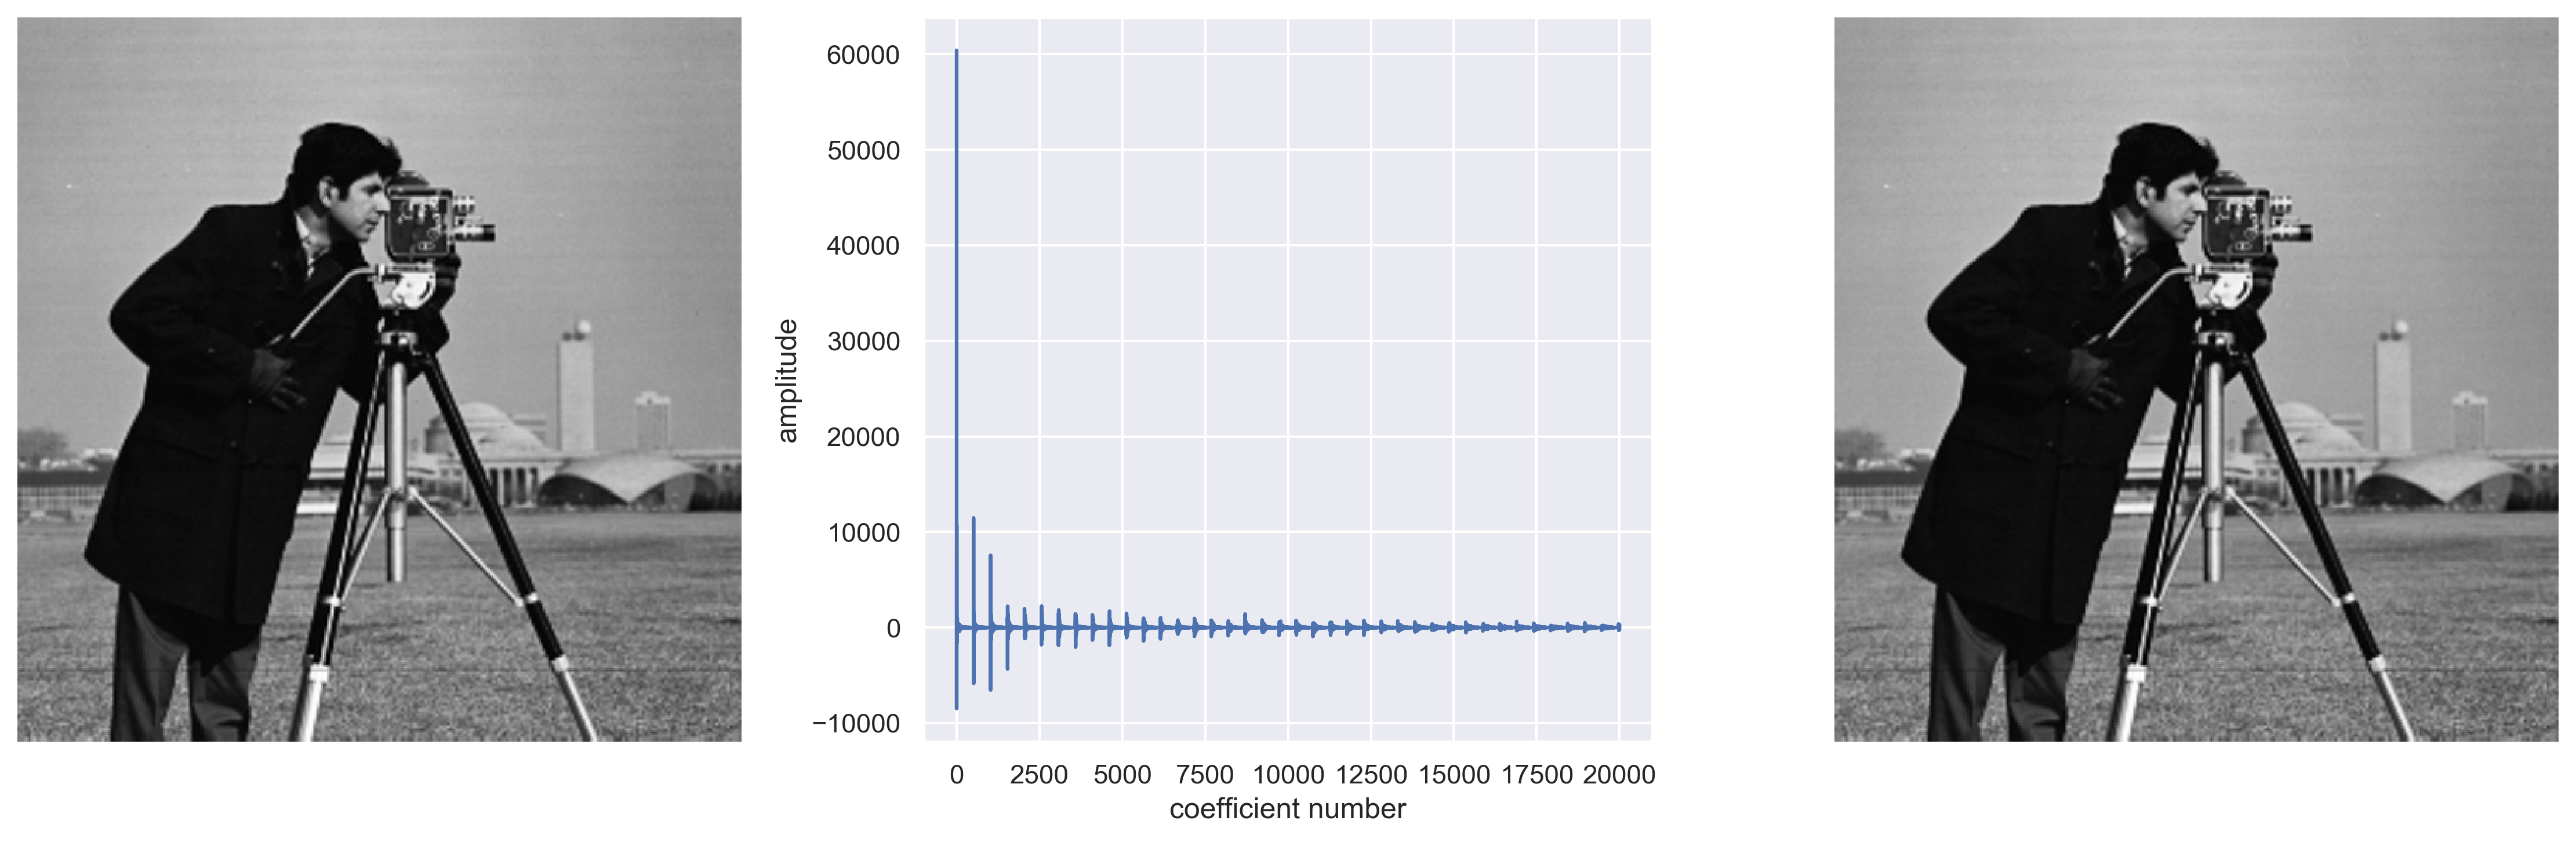
\includegraphics[width=\textwidth]{C2-sparsity.png}
	\caption{Original $512 \times 512$, 8-bit image (left), and its first 20,000 DCT coefficients (middle). Most of the signal energy is concentrated in just a few of the coefficients that are close to the origin. By discarding all but the first 25,000 coefficients and then inverting it, the resulting image (right) is perceptually no different from the original.}
	\label{fig:sparsity}
\end{figure}